\section{Stereo vision}

Three-dimensional dynamic capture means in general the way of recording a sequence of movements of a real-life target or scene.
This section introduces the methods for seeing three-dimensional structures from stereo setups, consisting of two or more cameras.
The configuration of a proper setup with two is described; it can be extended to the multi-view domain.
The previous section described how to record a view of a scene with a camera. From now on, the term camera refers to a particular camera configuration, which can be a single physical camera moved to different locations.

\subsection{Coordinate systems and transforms} \label{sec:coord}

The camera is a projective object located somewhere in the imaged scene.
Its \textit{intrinsic parameters} model the properties of projection, but do not take into account the camera location in any global coordinate system.
The \textit{extrinsic parameters} contain the camera location and rotation in another global coordinate system, structured as a matrix.
This is especially advantageous when there are more than one cameras and their coordinates must be related.
\cite{hartley03multiview,heyden2005multiple}
This part quickly reviews basic transforms whose results are needed in the later reconstruction steps.

%Calibration is often specified with a camera projection matrix, or several separate matrices.
%It may be convenient to store intrinsics and extrinsics separately if the intrinsic matrix is constant for several pictures, for example.


\simplefig{h}{%
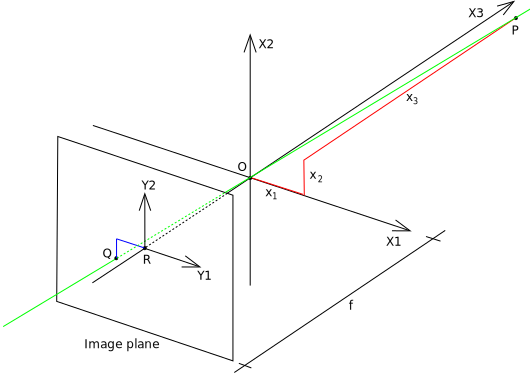
\includegraphics[width=0.7\textwidth]{gfx/pinhole3d}
}{fig:pinhole3d}
{Pinhole camera geometry. Camera coordinate system origin at O, axis X3 points towards the optical axis, Y1 and Y2 point to image plane axes and R is the principal point, at the image center. The point P projects to Q, as well as everything else on the line joining them. The image plane is f units away from camera origin; f is called the focal length.}

In computer graphics and vision, points and directions are usually described in homogeneous coordinates. \cite{dubrofsky2009homography,hartley03multiview} Translation, perspective projection, rotation, and other operations are conveniently described by using an additional dimension, of which usually the last element is 1: $(x, y, z, 1)$. All points $(xw, yw, zw, w)$ map to the same point $(x, y, z)$.

%Homography definition (mapping of points and lines in $P^2$)

The imaging process essentially captures a projection to a flat two-dimensional plane of the camera's view, as described in section \ref{sec:imaging}.
When relating points between different cameras that view the same scene, the cameras' relational positions and rotations must be known.
One of the cameras is often conveniently chosen as the origin of a global coordinate frame, so that its extrinsic parameters become unity transforms (programming libraries often assume this, see e.g. \cite{opencv}).
Each three-dimensional point in the world is transformed to the small sensor or film inside the camera, which is then digitized to a discrete two-dimensional grid of pixels. The size of this pixel array (i.e. image) is referred to as the camera's resolution.

%Figure \ref{fig:TODO} illustrates this transformation chain, which is encoded as the following equations, given a homogeneous point (4-dimensional vector) $X$ representing a 3D location described in physical (e.g. metric) coordinates:

The transformation chain is encoded as follows, given a homogeneous point (4-dimensional vector) $X$ representing a 3D location described in physical (e.g. metric) coordinates:

\begin{align}
	x &= P X\\
	  &= M_i X_s\\ % X_s on the sensor
	  &= M T R X\\
	  &= M_i M_p T R X\\ % R, T camera pose, M_4 to camera sensor, M_3 to pixel coords
\end{align}

$x$ is a 2d pixel in a discrete image, $X_s$ exists on the sensor. $R$, $T$ encode the camera rotation and translation (extrinsics); $M_p$ projects the world coordinates to the camera sensor (film) - still in world coordinates (intrinsics!), and finally the affine $M_i$ transforms the points from the sensor to pixel coordinates on the digital discretized image.

The whole projection $P = M_i M_p T R$ can be used as-is without decomposing it to separate matrices, unless the individual parameters are needed. As the chain consists of several matrices, some of them are defined only up to scale; the coordinate systems' units can be chosen freely. Software packages usually do not decompose the chain, because it is not needed and unique parameters cannot be found because of scaling.

%The external camera parameters are called the extrinsics: camera coordinate system position and rotation (heading) in the global space.
%Camera position sits at the projection center blah.

The internal parameters, intrinsics, encode how the image is formed on the sensor: they consist of focal length, sensor size and principal point:

\begin{equation}
	M =
	\begin{pmatrix}
		m_x & \gamma & u_0\\
		0   &    m_y & v_0\\
		0   &        0 & 1
	\end{pmatrix}
\cdot
	\begin{pmatrix}
		f & 0 & 0\\
		0 & f & 0\\
		0 & 0 & 1
	\end{pmatrix}
	=
	\begin{pmatrix}
		\alpha_x & \gamma   & u_0\\
		0        & \alpha_y & v_0\\
		0        & 0        & 1
	\end{pmatrix}
\end{equation}

For simplicity, it is often denoted $\alpha_x = m_x f$, $\alpha_y = m_y f$. $R = (u_0, v_0)$ is the image center (or principal point). For square pixels, $m_x = m_y$, and for a non-skewed sensor, $\gamma = 0$, which is often the case. \cite{hartley03multiview,szeliski10vision,heyden2005multiple}

%Le image. Horizontal planar triangle, lines between camera origins etc. lecture11.pdf.

\subsection{Camera calibration}

%In order to accurately measure a scene with a camera, the camera's properties must be known.
Reconstruction algorithms need to relate points between images; the camera properties are needed.
Calibrating a camera means to measure its intrinsics and extrinsics in order to map its data to a known coordinate frame.
Calibration has always to be done, but it does not necessary need to be a manual step before scanning; self-calibration attempts to target this convenience problem. \cite{pollefeys1999hand,hartley03multiview}

%Projective calibration only is too general, as it leaves out some assumptions that can be done about a physical world, such as relative angles and sizes; metric calibration something something. \cite{zisserman1995metric}.

Automatic calibration tools rely on an amount of feature pairs of which the best matches are found, or a known pattern, such as a planar checkerboard pattern [chuan; zhang] whose features are also distinguished with a similar algorithm but a priori knowledge of the object structure is used for precise calibration.
These usually need several pictures taken with the same camera from different poses.

The checkerboard calibration step can also measure optical distortion at the same time. \cite{opencv,camcalmatlab}

%TODO Figure: show extrinsic in matlab cam calibs, nice pics (both cam and world centered)

%Single three-dimensional calibration object is also sufficient blbl

One possible way is direct linear transform (DLT)
\cite{hartley03multiview}: the whole matrix $P$ is solved from $x = PX$ by constructing a system of equations from the projections, and minimizing an error metric, as the case is usually overconditioned.

%Methods that dig the matrix out of a single image have certain restrictions, and won't work if e.g. seven points lie on the same plane [longuet-higgins etc.]

%XXX see below. Intrinsic, extrinsic. Distortions. Projection matrices. Camera resectioning.

%many single planar chessboard pics vs. a single image of an accurate 3d model.

%The scale of values in the equations above affects the precision [hartley, in defense of .., h,ziss]. A similarity transform can be used to modify the values to a more consistent range; this is called normalization of the data.


\subsection{Binocular disparity}
%Essential, fundamental matrices. Correspondence problem. Rectification, undistortion. Epipolar geometry.

\simplefig{h!}{
\begin{tikzpicture}[scale=0.3]
	% P, Z
	\draw[fill] (0, 20) circle [radius=0.3];
	\node at (0, 21) {$P$};

	\draw [<->] (0, 0.5) -- (0, 19.5);
	\node at (0.5, 10) {$Z$};

	% origins, T
	% TODO: circles, node ends not exactly at those points
	\draw [<->] (-9.5,0) -- (9.5, 0);
	\draw[fill] (-10, 0) circle [radius=0.3];
	\draw[fill] ( 10, 0) circle [radius=0.3];
	\node at (-10, -1) {$O_l$};
	\node at (10, -1) {$O_r$};
	\node at (0, -1) {$T$};

	% headings
	\draw [->] (-10, 0) -- (-10, 10);
	\draw [->] (10, 0) -- (10, 10);

	% image planes, at y=4
	\draw[thick] (-13, 4) -- (-7, 4);
	\draw[thick] (13, 4) -- (7, 4);

	\draw [<->] (-6, 0.5) -- (-6, 3.5);
	\node at (-5.5, 2) {$f$};


	% intersection points at principals and xs
	\draw[fill] (-10, 4) circle [radius=0.3];
	\draw[fill] (10, 4) circle [radius=0.3];

	\node at (-10.5, 3) {$c_l$};
	\node at (10.5, 3) {$c_r$};

	\node at (-9, 5) {$x_l$};
	\node at (9, 5) {$x_r$};


	% O-to-P
	\draw (-10, 0) -- (0, 20);
	\draw (10, 0) -- (0, 20);


	% p
	\draw[fill] (8, 4) circle [radius=0.3];
	\node at (8, 3) {$p_r$};
	\draw[fill] (-8, 4) circle [radius=0.3];
	\node at (-8, 3) {$p_l$};
\end{tikzpicture}
}{fig:simplestereo}
{A very simple stereo setup, picture from above. The image planes (thick lines) are actually imaginary, as a real film in a camera would exist behind the principal point and project the image upside down, as described earlier in \ref{sec:imaging}. The coordinates exist in the world coordinate units. The symbols $O$ are the camera origins ($T$ units between each other); $c$ the principal points; $x$ the image plane coordinates of $p$ w.r.t. the principal points; and $f$ is the focal length. The unknown is $Z$, depth of point $P$.}

%Next, the setup of binocular stereo vision is described. Common stereo vision rigs use the simplest possible case: two identical cameras with a fixed distance, both oriented to the same direction, parallel to the line connecting them, as in figure \ref{fig:simplestereo}.

Assuming known calibration with identical cameras (same focal length and sensor) in a setup described above, visualized in figure \ref{fig:simplestereo}, points can be triangulated as follows:

From similar triangles with a common vertex at $P$, we get (note that $x_r < 0$ as it's to the left, towards to the negative axis, from the corresponding plane's origin)

\begin{align}
	\frac{Z}{T} &= \frac{Z-f}{T - x_l + x_r} \\
	&= \frac{Z-f}{T - d}\\
	ZT - Zd &= ZT - fT\\
	Z &= \frac{fT}{d} \label{eq:z}
\end{align}

The disparity $d$ is the difference of the points in their image planes, $d = x_r - x_l$.
If the image planes would be fixed as being physically correct, in the back side of the camera origins, the focal length should be negated to keep the correct interpretation and sign because the projected physical image is mirrored in both axes. Image processing between the sensor and a picture file usually inverts this.

As the equation \ref{eq:z} shows, depth is directly inversely proportional to disparity in this simple case.
To map the depth to correct units, only focal length $f$ and the baseline $T$ are needed additionally; when using pixel coordinates instead of physical in $d$, also the pixel size should be taken into account.
All of these are encoded in the camera parameters.
Algorithms such as those in OpenCV \cite{opencv} can compute point clouds from disparity images.

\subsection{Epipolar geometry}

\simplefig{h!}{
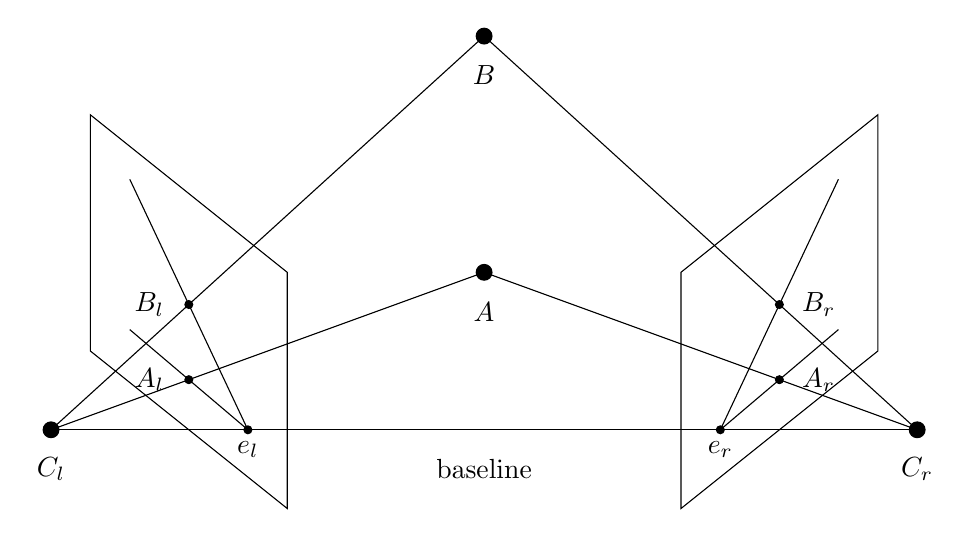
\begin{tikzpicture}[scale=0.5]
	% cameras
	\draw[fill] (-11,-1) circle [radius=0.2];
	\draw[fill] ( 11,-1) circle [radius=0.2];
	\draw (-11,-1) -- (11, -1);
	\node at (0, -2) { baseline };

	\node at (-11,-2) {$C_l$};
	\node at ( 11,-2) {$C_r$};

	% planes
	\draw (-10,1) -- (-10,7) -- (-5,3) -- (-5,-3) -- cycle;
	\draw ( 10,1) -- ( 10,7) -- ( 5,3) -- ( 5,-3) -- cycle;

	% 3d pts
	\draw[fill] ( 0,3) circle [radius=0.2];
	\draw[fill] ( 0,9) circle [radius=0.2];
	\node at (0,2) {$A$};
	\node at (0,8) {$B$};

	% origins via pts
	\draw (-11,-1) -- (0,3) -- (11,-1);
	\draw (-11,-1) -- (0,9) -- (11,-1);

	% epis
	\draw[fill] (-6,-1) circle [radius=0.1];
	\draw[fill] (6,-1) circle [radius=0.1];
	\node at (-6,-1.5) { $e_l$ };
	\node at (6,-1.5) { $e_r$ };

	% projections
	\draw[fill] (-7.5,0.2727) circle [radius=0.1];
	\draw[fill] (-7.5,2.1818) circle [radius=0.1];
	\node at (-8.5, 0.2727) {$A_l$};
	\node at (-8.5, 2.1818) {$B_l$};
	% lines from epis
	\draw (-6,-1) -- +(-2*1.5,2*1.2727);%(-7.5,0.2727);
	\draw (-6,-1) -- +(-2*1.5,2*3.1818);%(-7.5,2.1818);

	\draw[fill] (7.5,0.2727) circle [radius=0.1];
	\draw[fill] (7.5,2.1818) circle [radius=0.1];
	\node at (8.5, 0.2727) {$A_r$};
	\node at (8.5, 2.1818) {$B_r$};
	\draw (6,-1) -- +(2*1.5,2*1.2727);%(7.5,0.2727);
	\draw (6,-1) -- +(2*1.5,2*3.1818);%(7.5,2.1818);
\end{tikzpicture}
}{fig:epigeom}
{Two camera views on same scene.
World points $A$, $B$ project to planes of different views imaged from $C_l$ and $C_r$ on the left ($A_l$ and $B_l$), and to the right ($A_r$, $B_r$).
When $A_l$ is known, its corresponding point $A_r$ (not initially known in practice) is found on the epipolar line joining $e_r$ and $A_r$ in the right image.
All epipolar lines in a view join in the same point ($e_l$ and $e_r$).}

Triangulation or reconstruction of the scene structure given by image pair(s) is usually done on the base of a known relationship between the cameras.
Such relationship, known as calibrating the cameras, can be automatically determined, given by corresponding points that can be distinguished in each image and matched.
\cite{trucco1998introductory,hartley03multiview}

In stereo vision, the same scene of interest is seen by two or more cameras at the same time.
The cameras are rarely aligned perfectly such as in the disparity setup described above, however.
Epipolar geometry encodes the relations between arbitrarily positioned cameras in a standard way so that coordinates of a 3D point seen in several images can be calculated with the same triangulation.

A point seen by camera $C_l$ at 3D point A could be anywhere on the line between $C_l$'s origin and P, because a certain line passing through the principal point always projects to a point.
This line is seen as a single point $A_l$.
From another viewpoint in camera $C_r$, this line equals to some line on B's image plane.
The real point must be on that line.
The inverse applies for any point on $C_r$ and a line on $C_l$.
The lines on the image planes are called epipolar lines.

Essential matrix defines how the camera poses differ by the something something points seen by both. When $A_l$, $A_r$ encode the points in figure \ref{fig:epigeom} by the corresponding camera coordinates, and the baseline difference (vector from $C_l$ to $C_r$) is marked as $t$, it holds that $(A_l-C_l) \cdot t \times (A_r-C_r) = 0$, as all the vectors are coplanar; the cross product yields a normal to the plane, which is perpendicular to all the vectors, thus the dot product equals 0. \cite{hartley03multiview}

Essential matrix is a matrix form of this relation; it includes the relative rotation and translation of the two cameras.

%\begin{align*} \label{eq:essential}
%	%A_r &= R (A_l - t) \\
%	%A_r^T R T A_l &= 0 \\
%	%A_r^T E A_l &= 0
%	A_l \cdot t \times A_r = 0\\
%	A_l \cdot t \times R A_r = 0\\
%	A_l^T T
%\end{align*}

%where $T$ is the cross-product form of $t$ encoded in a matrix form as below. The essential matrix is obtained as $E = R T$.
%
%Le image. lecture11.pdf. O->p dot (O->O' cross O'->p') = 0
%
%Cross product expressed in a skew-symmetric matrix form is
%\begin{equation}
%\vec a \times \vec b =
%\begin{pmatrix}
%	 0   & -a_z &  a_y\\
%	 a_z &  0   & -a_x\\
%	-a_y &  a_x & 0
%\end{pmatrix}
%\begin{pmatrix}
%	b_x\\b_y\\b_z
%\end{pmatrix}
%= \vec c
%\end{equation}

Fundamental matrix relates the corresponding points in stereo images; it has the same meaning as the essential matrix, but it works in the pixel coordinates of the cameras, which are obtained after the projective transform that takes the intrinsics into account.

Inverting the matrix $M_i$ (\ref{sec:coord}) in sensor-to-pixel coordinate transform and using it on pixel coordinates, world coordinates seen by the camera can be obtained.

%\[
%\hat pAl = M_p A_l\\
%\hat A_r = M_p A_r
%\]
%
%and using it on pixel coordinates, the world coords can be obtained, plugging in to the equation \ref{eq:essential}
%
%\[
%A_r^T E A_l = 0\\
%(M_p^-1 \hat A_r)^T E (M_p^-1 \hat A_l) = 0\\
%\hat A_r^T M_p^-T E M_p^-1 A_l = 0\\
%\hat A_r^T F \hat A_l = 0
%\]
%
%the fundamental matrix
%
%\[
%F = M_p^-T E M_p^-1 = M_p^-T R T M_p^-1
%\]

The fundamental matrix relates the pixels and epipolar lines, and as such it is useful in image processing where the images are described as pixels in a color array (image) and not colored physical coordinates.

%Epipole can be interpreted as the location of another camera as seen by other camera.

\subsection{Point matching}

Previously, basics for reconstructing three-dimensional location for a point pair were introduced, assuming known positions for the same point in different images.
To reconstruct a whole scene from a full image, all pairwise points must be matched, i.e. found that what pixel in one view represents the same object as one in other view.

Matching is often also called correspondence searching:
Given a pixel in one image, what is the corresponding pixel in another image taken from the same scene?

Matching can be done in sparse or dense mode; sparse matching finds a set of \textit{features} from each image, and tries to match them. Dense matching runs through each pixel of one image and tries to find the same from another one with e.g. template matching \cite{?}; from the coordinate differences in image space between the two images, a disparity map is built. The disparities can be directly transformed to depth values.

The sparse points from the feature locations are found with an algorithm such as SIFT [?], SURF [?] or Harris corner detector [?].

\subsection{Correspondence and rectification} \label{sec:rectification}

In order to triangulate a real point from two or more photos, the location of the point in all images must be known.
Rectification is a process that simplifies this search problem by restricting the search to a single dimension.
By aligning the cameras such that their images are coplanar, the search only has to be performed on a line that is parallel to the line connecting the camera centers.
After rectification, the corresponding lines are axis-aligned (horizontal or vertical) in both images. \cite{hartley03multiview}
% LOL TODO guido gerig image rectification (stereo) slides

\subsection{N-view stereo}

It is also more computationally heavy, as more data must be processed; if no information about camera parameters is available, pairwise checks between the images may become expensive. \cite{wu2013towards}

The case of more cameras than a single pair uses the same principles in epipolar geometry. It brings more restrictions and dimensions; in three dimensions, for example, the fundamental matrix becomes three-dimensional, the trifocal tensor. \cite{hartley03multiview}

Multiple baseline stereo is a simple special case for many cameras. When all the cameras lie on the same baseline, calibration is easier and points can be selected by using a minimized sum of errors. \cite{okutomi1993multiple}

The cameras that are used in capturing a scene can be fixed or positioned arbitrarily; in fact, the structure from motion technique \cite{snavely2006photo,fitzgibbon1998automatic} enables to use just one camera that is moved around.
Accurate and fast reconstructions are still traditionally done with stereo camera pairs, though.

Another common way is to use pairwise cameras for individual reconstructions to build a point cloud for every pair, and then register them together. \cite{?}

%\subsection{Structure from motion}
%
%Structure from motion (SfM) refers usually to recovering the structure of a scene from the motion of a single camera.
%For each view, the pose of the camera is determined and the scene structure is extended with the new information in the image.
%(pollefeys)
%Bundle adjustment is used to refine the camera parameters.

%\subsection{Post-processing}
%Uv mapping. Manual work. 3d noise removal; ignore points that have no close pair in other clouds.
%Rendering: "as usual".
%Post: remodel the mesh (face), see what it would look like. Refine parameters to get a similar output as in the photos (normal map etc.), backproject. Use colors and highpass them; assume uniform lightning and locally uniform texture color (bradley). (Simply a rendering technique, that level of detail in 3D structure might not be needed). Still, structured light and/or shading assumptions [shape from single image cues/shading trucco,verri p.225] done too.


\subsection{Reprojection errors}

The quality of the reconstruction is measured by reprojecting the 3D points back to the cameras with the estimated parameters, and calculating the distance between the projected and original point. \cite{hartley03multiview}
Bundle adjustment \cite{wu2011multicore} seeks to optimize all camera parameters at once with good performance.

A common way to handle feature errors is Random Sample Consensus (RANSAC). Random subsets of the sample space is iterated, and samples that do not fit well to a model that is constructed of a smaller set are ignored. The iteration that matches most samples is selected. \cite{hartley03multiview}

